% Options for packages loaded elsewhere
\PassOptionsToPackage{unicode}{hyperref}
\PassOptionsToPackage{hyphens}{url}
\PassOptionsToPackage{dvipsnames,svgnames,x11names}{xcolor}
%
\documentclass[
  letterpaper,
  DIV=11,
  numbers=noendperiod]{scrartcl}

\usepackage{amsmath,amssymb}
\usepackage{iftex}
\ifPDFTeX
  \usepackage[T1]{fontenc}
  \usepackage[utf8]{inputenc}
  \usepackage{textcomp} % provide euro and other symbols
\else % if luatex or xetex
  \usepackage{unicode-math}
  \defaultfontfeatures{Scale=MatchLowercase}
  \defaultfontfeatures[\rmfamily]{Ligatures=TeX,Scale=1}
\fi
\usepackage{lmodern}
\ifPDFTeX\else  
    % xetex/luatex font selection
\fi
% Use upquote if available, for straight quotes in verbatim environments
\IfFileExists{upquote.sty}{\usepackage{upquote}}{}
\IfFileExists{microtype.sty}{% use microtype if available
  \usepackage[]{microtype}
  \UseMicrotypeSet[protrusion]{basicmath} % disable protrusion for tt fonts
}{}
\makeatletter
\@ifundefined{KOMAClassName}{% if non-KOMA class
  \IfFileExists{parskip.sty}{%
    \usepackage{parskip}
  }{% else
    \setlength{\parindent}{0pt}
    \setlength{\parskip}{6pt plus 2pt minus 1pt}}
}{% if KOMA class
  \KOMAoptions{parskip=half}}
\makeatother
\usepackage{xcolor}
\setlength{\emergencystretch}{3em} % prevent overfull lines
\setcounter{secnumdepth}{-\maxdimen} % remove section numbering
% Make \paragraph and \subparagraph free-standing
\ifx\paragraph\undefined\else
  \let\oldparagraph\paragraph
  \renewcommand{\paragraph}[1]{\oldparagraph{#1}\mbox{}}
\fi
\ifx\subparagraph\undefined\else
  \let\oldsubparagraph\subparagraph
  \renewcommand{\subparagraph}[1]{\oldsubparagraph{#1}\mbox{}}
\fi

\usepackage{color}
\usepackage{fancyvrb}
\newcommand{\VerbBar}{|}
\newcommand{\VERB}{\Verb[commandchars=\\\{\}]}
\DefineVerbatimEnvironment{Highlighting}{Verbatim}{commandchars=\\\{\}}
% Add ',fontsize=\small' for more characters per line
\usepackage{framed}
\definecolor{shadecolor}{RGB}{241,243,245}
\newenvironment{Shaded}{\begin{snugshade}}{\end{snugshade}}
\newcommand{\AlertTok}[1]{\textcolor[rgb]{0.68,0.00,0.00}{#1}}
\newcommand{\AnnotationTok}[1]{\textcolor[rgb]{0.37,0.37,0.37}{#1}}
\newcommand{\AttributeTok}[1]{\textcolor[rgb]{0.40,0.45,0.13}{#1}}
\newcommand{\BaseNTok}[1]{\textcolor[rgb]{0.68,0.00,0.00}{#1}}
\newcommand{\BuiltInTok}[1]{\textcolor[rgb]{0.00,0.23,0.31}{#1}}
\newcommand{\CharTok}[1]{\textcolor[rgb]{0.13,0.47,0.30}{#1}}
\newcommand{\CommentTok}[1]{\textcolor[rgb]{0.37,0.37,0.37}{#1}}
\newcommand{\CommentVarTok}[1]{\textcolor[rgb]{0.37,0.37,0.37}{\textit{#1}}}
\newcommand{\ConstantTok}[1]{\textcolor[rgb]{0.56,0.35,0.01}{#1}}
\newcommand{\ControlFlowTok}[1]{\textcolor[rgb]{0.00,0.23,0.31}{#1}}
\newcommand{\DataTypeTok}[1]{\textcolor[rgb]{0.68,0.00,0.00}{#1}}
\newcommand{\DecValTok}[1]{\textcolor[rgb]{0.68,0.00,0.00}{#1}}
\newcommand{\DocumentationTok}[1]{\textcolor[rgb]{0.37,0.37,0.37}{\textit{#1}}}
\newcommand{\ErrorTok}[1]{\textcolor[rgb]{0.68,0.00,0.00}{#1}}
\newcommand{\ExtensionTok}[1]{\textcolor[rgb]{0.00,0.23,0.31}{#1}}
\newcommand{\FloatTok}[1]{\textcolor[rgb]{0.68,0.00,0.00}{#1}}
\newcommand{\FunctionTok}[1]{\textcolor[rgb]{0.28,0.35,0.67}{#1}}
\newcommand{\ImportTok}[1]{\textcolor[rgb]{0.00,0.46,0.62}{#1}}
\newcommand{\InformationTok}[1]{\textcolor[rgb]{0.37,0.37,0.37}{#1}}
\newcommand{\KeywordTok}[1]{\textcolor[rgb]{0.00,0.23,0.31}{#1}}
\newcommand{\NormalTok}[1]{\textcolor[rgb]{0.00,0.23,0.31}{#1}}
\newcommand{\OperatorTok}[1]{\textcolor[rgb]{0.37,0.37,0.37}{#1}}
\newcommand{\OtherTok}[1]{\textcolor[rgb]{0.00,0.23,0.31}{#1}}
\newcommand{\PreprocessorTok}[1]{\textcolor[rgb]{0.68,0.00,0.00}{#1}}
\newcommand{\RegionMarkerTok}[1]{\textcolor[rgb]{0.00,0.23,0.31}{#1}}
\newcommand{\SpecialCharTok}[1]{\textcolor[rgb]{0.37,0.37,0.37}{#1}}
\newcommand{\SpecialStringTok}[1]{\textcolor[rgb]{0.13,0.47,0.30}{#1}}
\newcommand{\StringTok}[1]{\textcolor[rgb]{0.13,0.47,0.30}{#1}}
\newcommand{\VariableTok}[1]{\textcolor[rgb]{0.07,0.07,0.07}{#1}}
\newcommand{\VerbatimStringTok}[1]{\textcolor[rgb]{0.13,0.47,0.30}{#1}}
\newcommand{\WarningTok}[1]{\textcolor[rgb]{0.37,0.37,0.37}{\textit{#1}}}

\providecommand{\tightlist}{%
  \setlength{\itemsep}{0pt}\setlength{\parskip}{0pt}}\usepackage{longtable,booktabs,array}
\usepackage{calc} % for calculating minipage widths
% Correct order of tables after \paragraph or \subparagraph
\usepackage{etoolbox}
\makeatletter
\patchcmd\longtable{\par}{\if@noskipsec\mbox{}\fi\par}{}{}
\makeatother
% Allow footnotes in longtable head/foot
\IfFileExists{footnotehyper.sty}{\usepackage{footnotehyper}}{\usepackage{footnote}}
\makesavenoteenv{longtable}
\usepackage{graphicx}
\makeatletter
\def\maxwidth{\ifdim\Gin@nat@width>\linewidth\linewidth\else\Gin@nat@width\fi}
\def\maxheight{\ifdim\Gin@nat@height>\textheight\textheight\else\Gin@nat@height\fi}
\makeatother
% Scale images if necessary, so that they will not overflow the page
% margins by default, and it is still possible to overwrite the defaults
% using explicit options in \includegraphics[width, height, ...]{}
\setkeys{Gin}{width=\maxwidth,height=\maxheight,keepaspectratio}
% Set default figure placement to htbp
\makeatletter
\def\fps@figure{htbp}
\makeatother
\newlength{\cslhangindent}
\setlength{\cslhangindent}{1.5em}
\newlength{\csllabelwidth}
\setlength{\csllabelwidth}{3em}
\newlength{\cslentryspacingunit} % times entry-spacing
\setlength{\cslentryspacingunit}{\parskip}
\newenvironment{CSLReferences}[2] % #1 hanging-ident, #2 entry spacing
 {% don't indent paragraphs
  \setlength{\parindent}{0pt}
  % turn on hanging indent if param 1 is 1
  \ifodd #1
  \let\oldpar\par
  \def\par{\hangindent=\cslhangindent\oldpar}
  \fi
  % set entry spacing
  \setlength{\parskip}{#2\cslentryspacingunit}
 }%
 {}
\usepackage{calc}
\newcommand{\CSLBlock}[1]{#1\hfill\break}
\newcommand{\CSLLeftMargin}[1]{\parbox[t]{\csllabelwidth}{#1}}
\newcommand{\CSLRightInline}[1]{\parbox[t]{\linewidth - \csllabelwidth}{#1}\break}
\newcommand{\CSLIndent}[1]{\hspace{\cslhangindent}#1}

\usepackage{booktabs}
\usepackage{longtable}
\usepackage{array}
\usepackage{multirow}
\usepackage{wrapfig}
\usepackage{float}
\usepackage{colortbl}
\usepackage{pdflscape}
\usepackage{tabu}
\usepackage{threeparttable}
\usepackage{threeparttablex}
\usepackage[normalem]{ulem}
\usepackage{makecell}
\usepackage{xcolor}
\usepackage{caption}
\KOMAoption{captions}{tableheading}
\makeatletter
\makeatother
\makeatletter
\makeatother
\makeatletter
\@ifpackageloaded{caption}{}{\usepackage{caption}}
\AtBeginDocument{%
\ifdefined\contentsname
  \renewcommand*\contentsname{Table of contents}
\else
  \newcommand\contentsname{Table of contents}
\fi
\ifdefined\listfigurename
  \renewcommand*\listfigurename{List of Figures}
\else
  \newcommand\listfigurename{List of Figures}
\fi
\ifdefined\listtablename
  \renewcommand*\listtablename{List of Tables}
\else
  \newcommand\listtablename{List of Tables}
\fi
\ifdefined\figurename
  \renewcommand*\figurename{Figure}
\else
  \newcommand\figurename{Figure}
\fi
\ifdefined\tablename
  \renewcommand*\tablename{Table}
\else
  \newcommand\tablename{Table}
\fi
}
\@ifpackageloaded{float}{}{\usepackage{float}}
\floatstyle{ruled}
\@ifundefined{c@chapter}{\newfloat{codelisting}{h}{lop}}{\newfloat{codelisting}{h}{lop}[chapter]}
\floatname{codelisting}{Listing}
\newcommand*\listoflistings{\listof{codelisting}{List of Listings}}
\makeatother
\makeatletter
\@ifpackageloaded{caption}{}{\usepackage{caption}}
\@ifpackageloaded{subcaption}{}{\usepackage{subcaption}}
\makeatother
\makeatletter
\@ifpackageloaded{tcolorbox}{}{\usepackage[skins,breakable]{tcolorbox}}
\makeatother
\makeatletter
\@ifundefined{shadecolor}{\definecolor{shadecolor}{rgb}{.97, .97, .97}}
\makeatother
\makeatletter
\makeatother
\makeatletter
\makeatother
\ifLuaTeX
\usepackage[bidi=basic]{babel}
\else
\usepackage[bidi=default]{babel}
\fi
\babelprovide[main,import]{english}
% get rid of language-specific shorthands (see #6817):
\let\LanguageShortHands\languageshorthands
\def\languageshorthands#1{}
\ifLuaTeX
  \usepackage{selnolig}  % disable illegal ligatures
\fi
\IfFileExists{bookmark.sty}{\usepackage{bookmark}}{\usepackage{hyperref}}
\IfFileExists{xurl.sty}{\usepackage{xurl}}{} % add URL line breaks if available
\urlstyle{same} % disable monospaced font for URLs
\hypersetup{
  pdftitle={Model selection},
  pdfauthor={Daniela Palleschi},
  pdflang={en},
  colorlinks=true,
  linkcolor={blue},
  filecolor={Maroon},
  citecolor={Blue},
  urlcolor={Blue},
  pdfcreator={LaTeX via pandoc}}

\title{Model selection}
\usepackage{etoolbox}
\makeatletter
\providecommand{\subtitle}[1]{% add subtitle to \maketitle
  \apptocmd{\@title}{\par {\large #1 \par}}{}{}
}
\makeatother
\subtitle{Parsimonious model selection}
\author{Daniela Palleschi}
\date{2024-02-09}

\begin{document}
\maketitle
\ifdefined\Shaded\renewenvironment{Shaded}{\begin{tcolorbox}[boxrule=0pt, interior hidden, breakable, borderline west={3pt}{0pt}{shadecolor}, frame hidden, enhanced, sharp corners]}{\end{tcolorbox}}\fi

\renewcommand*\contentsname{Table of contents}
{
\hypersetup{linkcolor=}
\setcounter{tocdepth}{3}
\tableofcontents
}
\hypertarget{learning-objectives}{%
\section*{Learning Objectives}\label{learning-objectives}}

Today we will\ldots{}

\begin{itemize}
\tightlist
\item
  apply remedies for nonconvergence
\item
  reduce our RES with a data-driven approach
\item
  compare a parsimonious model to maximal and intercept-only models
\end{itemize}

\hypertarget{resources}{%
\section*{Resources}\label{resources}}

\begin{itemize}
\tightlist
\item
  this lecture covers

  \begin{itemize}
  \tightlist
  \item
    Sections 10.3-5 in Sonderegger (2023)
  \item
    Section 15.7.3 `Convergence Issues' in Winter (2019)
  \item
    Brauer \& Curtin (2018)
  \item
    Meteyard \& Davies (2020)
  \end{itemize}
\item
  we will continue using the data from Biondo et al. (2022)
\end{itemize}

\hypertarget{set-up}{%
\section*{Set-up}\label{set-up}}
\addcontentsline{toc}{section}{Set-up}

\begin{Shaded}
\begin{Highlighting}[]
\CommentTok{\# suppress scientific notation}
\FunctionTok{options}\NormalTok{(}\AttributeTok{scipen=}\DecValTok{999}\NormalTok{)}
\end{Highlighting}
\end{Shaded}

\begin{Shaded}
\begin{Highlighting}[]
\FunctionTok{library}\NormalTok{(broman)}
\CommentTok{\# function to format p{-}values}
\NormalTok{format\_pval }\OtherTok{\textless{}{-}} \ControlFlowTok{function}\NormalTok{(pval)\{}
\NormalTok{    dplyr}\SpecialCharTok{::}\FunctionTok{case\_when}\NormalTok{(}
\NormalTok{        pval }\SpecialCharTok{\textless{}}\NormalTok{ .}\DecValTok{001} \SpecialCharTok{\textasciitilde{}} \StringTok{"\textless{} .001"}\NormalTok{,}
\NormalTok{        pval }\SpecialCharTok{\textless{}}\NormalTok{ .}\DecValTok{01} \SpecialCharTok{\textasciitilde{}} \StringTok{"\textless{} .01"}\NormalTok{,}
\NormalTok{        pval }\SpecialCharTok{\textless{}}\NormalTok{ .}\DecValTok{05} \SpecialCharTok{\textasciitilde{}} \StringTok{"\textless{} .05"}\NormalTok{,}
        \ConstantTok{TRUE} \SpecialCharTok{\textasciitilde{}}\NormalTok{ broman}\SpecialCharTok{::}\FunctionTok{myround}\NormalTok{(pval, }\DecValTok{3}\NormalTok{)}
\NormalTok{    )}
\NormalTok{\}}
\end{Highlighting}
\end{Shaded}

\hypertarget{load-packages}{%
\subsection*{Load packages}\label{load-packages}}
\addcontentsline{toc}{subsection}{Load packages}

\begin{Shaded}
\begin{Highlighting}[]
\CommentTok{\# load libraries}
\NormalTok{pacman}\SpecialCharTok{::}\FunctionTok{p\_load}\NormalTok{(}
\NormalTok{               tidyverse,}
\NormalTok{               here,}
\NormalTok{               janitor,}
               \CommentTok{\# new packages for mixed models:}
\NormalTok{               lme4,}
\NormalTok{               lmerTest,}
\NormalTok{               broom.mixed,}
\NormalTok{               lattice)}
\end{Highlighting}
\end{Shaded}

\begin{Shaded}
\begin{Highlighting}[]
\NormalTok{lmer }\OtherTok{\textless{}{-}}\NormalTok{ lmerTest}\SpecialCharTok{::}\NormalTok{lmer}
\end{Highlighting}
\end{Shaded}

\hypertarget{load-data}{%
\subsection*{Load data}\label{load-data}}
\addcontentsline{toc}{subsection}{Load data}

\begin{itemize}
\tightlist
\item
  data from Biondo et al. (2022)
\end{itemize}

\begin{Shaded}
\begin{Highlighting}[]
\NormalTok{df\_biondo }\OtherTok{\textless{}{-}}
  \FunctionTok{read\_csv}\NormalTok{(}\FunctionTok{here}\NormalTok{(}\StringTok{"data"}\NormalTok{, }\StringTok{"Biondo.Soilemezidi.Mancini\_dataset\_ET.csv"}\NormalTok{),}
           \AttributeTok{locale =} \FunctionTok{locale}\NormalTok{(}\AttributeTok{encoding =} \StringTok{"Latin1"}\NormalTok{) }\DocumentationTok{\#\# for special characters in Spanish}
\NormalTok{           ) }\SpecialCharTok{|\textgreater{}} 
  \FunctionTok{clean\_names}\NormalTok{() }\SpecialCharTok{|\textgreater{}} 
  \FunctionTok{mutate}\NormalTok{(}\AttributeTok{gramm =} \FunctionTok{ifelse}\NormalTok{(gramm }\SpecialCharTok{==} \StringTok{"0"}\NormalTok{, }\StringTok{"ungramm"}\NormalTok{, }\StringTok{"gramm"}\NormalTok{)) }\SpecialCharTok{|\textgreater{}} 
  \FunctionTok{mutate\_if}\NormalTok{(is.character,as\_factor) }\SpecialCharTok{|\textgreater{}} \CommentTok{\# all character variables as factors}
  \FunctionTok{droplevels}\NormalTok{() }\SpecialCharTok{|\textgreater{}} 
  \FunctionTok{filter}\NormalTok{(adv\_type }\SpecialCharTok{==} \StringTok{"Deic"}\NormalTok{)}
\end{Highlighting}
\end{Shaded}

\hypertarget{set-contrasts}{%
\subsection{Set contrasts}\label{set-contrasts}}

\begin{Shaded}
\begin{Highlighting}[]
\FunctionTok{contrasts}\NormalTok{(df\_biondo}\SpecialCharTok{$}\NormalTok{verb\_t) }\OtherTok{\textless{}{-}} \FunctionTok{c}\NormalTok{(}\SpecialCharTok{{-}}\FloatTok{0.5}\NormalTok{,}\SpecialCharTok{+}\FloatTok{0.5}\NormalTok{)}
\FunctionTok{contrasts}\NormalTok{(df\_biondo}\SpecialCharTok{$}\NormalTok{gramm) }\OtherTok{\textless{}{-}} \FunctionTok{c}\NormalTok{(}\SpecialCharTok{{-}}\FloatTok{0.5}\NormalTok{,}\SpecialCharTok{+}\FloatTok{0.5}\NormalTok{)}
\end{Highlighting}
\end{Shaded}

\begin{Shaded}
\begin{Highlighting}[]
\FunctionTok{contrasts}\NormalTok{(df\_biondo}\SpecialCharTok{$}\NormalTok{verb\_t)}
\end{Highlighting}
\end{Shaded}

\begin{verbatim}
       [,1]
Past   -0.5
Future  0.5
\end{verbatim}

\begin{Shaded}
\begin{Highlighting}[]
\FunctionTok{contrasts}\NormalTok{(df\_biondo}\SpecialCharTok{$}\NormalTok{gramm)}
\end{Highlighting}
\end{Shaded}

\begin{verbatim}
        [,1]
gramm   -0.5
ungramm  0.5
\end{verbatim}

\hypertarget{start-maximal}{%
\section{Start maximal}\label{start-maximal}}

\begin{itemize}
\tightlist
\item
  model structure should be decided \emph{a priori}

  \begin{itemize}
  \tightlist
  \item
    included fixed (predictors and covariates) and random effects
  \end{itemize}
\end{itemize}

\hypertarget{maximal-model}{%
\subsection{Maximal model}\label{maximal-model}}

\begin{itemize}
\tightlist
\item
  starting point: most maximal model structure justified by your design

  \begin{itemize}
  \tightlist
  \item
    if this converges, great!
  \item
    if it doesn't, what does this mean and what should we do?
  \end{itemize}
\end{itemize}

\begin{Shaded}
\begin{Highlighting}[]
\NormalTok{fit\_verb\_fp\_mm }\OtherTok{\textless{}{-}} \FunctionTok{lmer}\NormalTok{(}\FunctionTok{log}\NormalTok{(fp) }\SpecialCharTok{\textasciitilde{}}\NormalTok{ verb\_t}\SpecialCharTok{*}\NormalTok{gramm }\SpecialCharTok{+} 
\NormalTok{                      (}\DecValTok{1} \SpecialCharTok{+}\NormalTok{ verb\_t}\SpecialCharTok{*}\NormalTok{gramm}\SpecialCharTok{|}\NormalTok{sj) }\SpecialCharTok{+}
\NormalTok{                      (}\DecValTok{1} \SpecialCharTok{+}\NormalTok{ verb\_t}\SpecialCharTok{*}\NormalTok{gramm}\SpecialCharTok{|}\NormalTok{item),}
                    \AttributeTok{data =}\NormalTok{ df\_biondo,}
                    \AttributeTok{subset =}\NormalTok{ roi }\SpecialCharTok{==} \DecValTok{4}\NormalTok{)}
\end{Highlighting}
\end{Shaded}

\begin{itemize}
\tightlist
\item
  we get a warning of singular fit
\end{itemize}

\hypertarget{convergence-issues}{%
\section{Convergence issues}\label{convergence-issues}}

\begin{itemize}
\tightlist
\item
  ``\emph{Convergence is not a metric of model quality}'' (Sonderegger,
  2023, p. 365, Box 10.2)

  \begin{itemize}
  \tightlist
  \item
    convergence does not always indicate ``overfitting'' or
    ``overparameterisation''
  \item
    can also be due to optimizer choice

    \begin{itemize}
    \tightlist
    \item
      since default optimizer was changed to \texttt{nloptwrap} from
      \texttt{bobyqa}, there seem to be more `false positive'
      convergence warnings
    \end{itemize}
  \end{itemize}
\item
  false-positive convergence: you get a convergence warning, but
  changing the optimizer and/or iteration count does not produce a
  warning
\item
  false-negative convergence: you do not get a warning, but your
  variance-covariance matrix might indicate overfitting
\end{itemize}

\hypertarget{nonconvergence-remedies}{%
\subsection{Nonconvergence remedies}\label{nonconvergence-remedies}}

\begin{itemize}
\tightlist
\item
  unfortunately there is no one ``right'' way to deal with convergence
  issues

  \begin{itemize}
  \tightlist
  \item
    important is to transparently report and justify your method
  \end{itemize}
\item
  Table 17 in Brauer \& Curtin (2018) (p.~404) suggests 20 remedies,
  whittled down to 10 suggestions in Sonderegger (2023)
\end{itemize}

\begin{figure}

{\centering 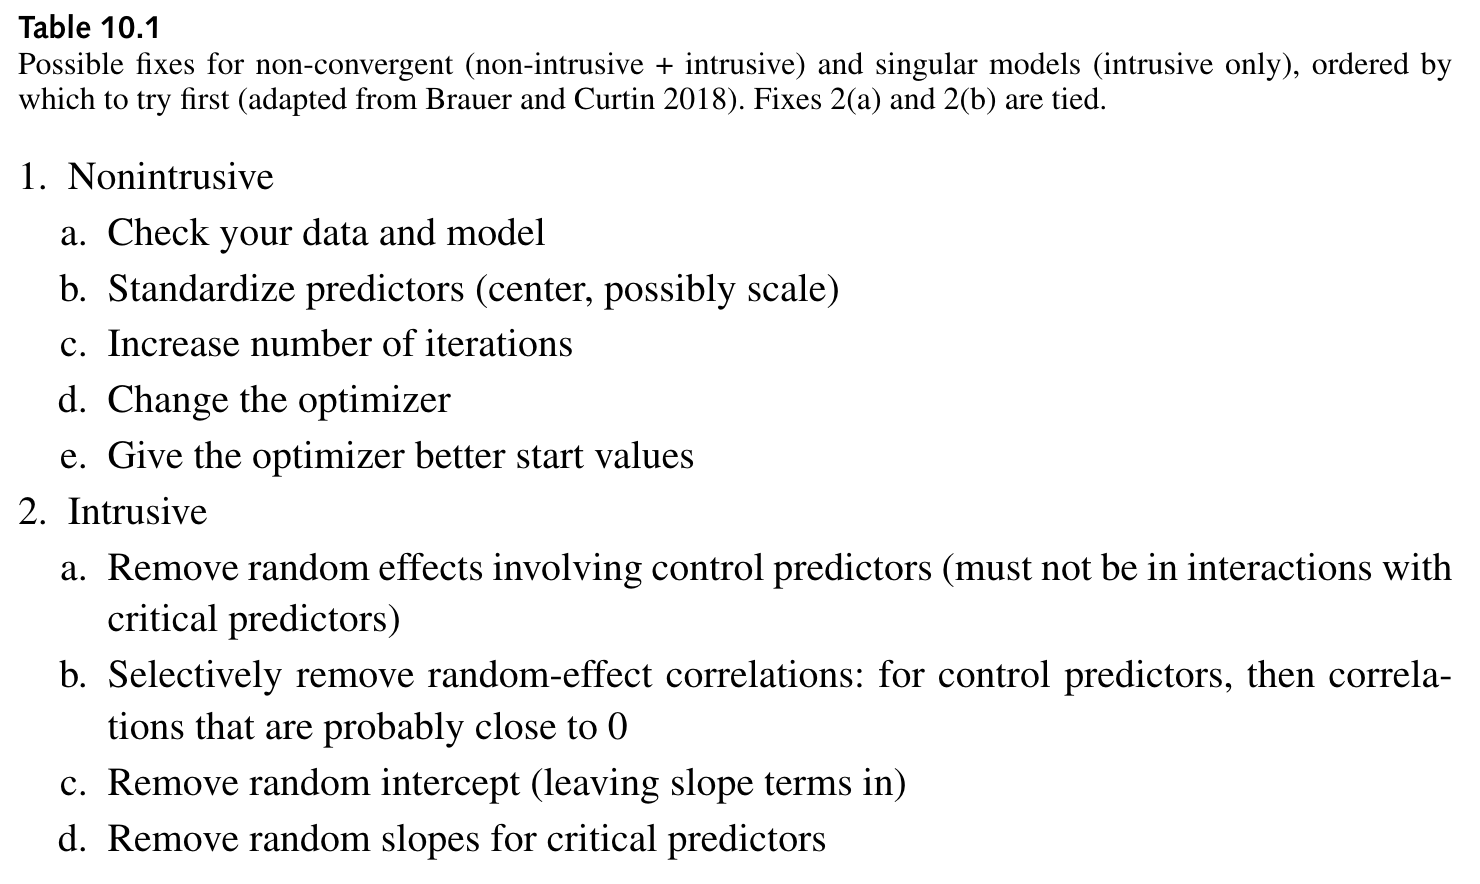
\includegraphics[width=4.93in,height=\textheight]{../../media/sonderegger_2023_convergence_table10.png}

}

\caption{\label{fig-table10}From Sonderegger (2023), p.~366}

\end{figure}

\hypertarget{intrusive-vs.-non-intrusive-remedies}{%
\subsection{Intrusive vs.~Non-intrusive
remedies}\label{intrusive-vs.-non-intrusive-remedies}}

\begin{itemize}
\item
  non-intrusive remedies amount to checking/adjusting data and model
  specifications
\item
  intrusive remedies involve reducing random effects structure

  \begin{itemize}
  \tightlist
  \item
    there are different schools of thought

    \begin{itemize}
    \tightlist
    \item
      random-intercepts only: increased Type I error rate =
      overconfident estimates
    \item
      maximal-but-singular-fit model (Barr et al., 2013): reduces power
      = underconfident estimates
    \item
      data-driven approach (Bates et al., 2015): can lose the forest for
      the trees, e.g., removing random slopes for predictors of interest
    \end{itemize}
  \end{itemize}
\item
  each strategy has its drawback

  \begin{itemize}
  \tightlist
  \item
    important is to choose your strategy \emph{a priori} and
    transparently report and justify your strategy
  \item
    even better: share/publish your data and code, which should be
    reproducible
  \end{itemize}
\end{itemize}

\hypertarget{convergence}{%
\subsection{\texorpdfstring{\texttt{?convergence}}{?convergence}}\label{convergence}}

\begin{itemize}
\tightlist
\item
  type \texttt{?convergence} in the Console and read the vignette

  \begin{itemize}
  \tightlist
  \item
    what suggestions does it make?
  \end{itemize}
\item
  compare this to \texttt{?isSingular}
\end{itemize}

\hypertarget{non-intrusive-methods}{%
\section{Non-intrusive methods}\label{non-intrusive-methods}}

\begin{itemize}
\tightlist
\item
  check your data structure/variables

  \begin{itemize}
  \tightlist
  \item
    check model assumptions (e.g., normality, missing transformations of
    variables)
  \item
    check your RES is justified by your experimental design/data
    structure
  \item
    centre your predictors (e.g., sum contrasts, or
    centring/standardizing) to reduce multicollinearity; reduces
    collinearity in the random effects (a possible source of
    nonconvergence)
  \item
    check observations per cell (e.g., is there a participant very few
    observations, or few observations per one condition? Should be at
    least \textgreater5 per cell)
  \end{itemize}
\item
  alter model controls:

  \begin{itemize}
  \tightlist
  \item
    increase iterations
  \item
    check optimizer
  \end{itemize}
\end{itemize}

\hypertarget{check-optimzer}{%
\subsection{Check optimzer}\label{check-optimzer}}

\begin{itemize}
\tightlist
\item
  optimizer

  \begin{itemize}
  \tightlist
  \item
    \texttt{lme4::allFit(model)} (can take a while to run)
  \end{itemize}
\end{itemize}

\begin{Shaded}
\begin{Highlighting}[]
\NormalTok{all\_fit\_verb\_fp\_mm }\OtherTok{\textless{}{-}} \FunctionTok{allFit}\NormalTok{(fit\_verb\_fp\_mm)}
\CommentTok{\# bobyqa : boundary (singular) fit: see help(\textquotesingle{}isSingular\textquotesingle{})}
\CommentTok{\# [OK]}
\CommentTok{\# Nelder\_Mead : [OK]}
\CommentTok{\# nlminbwrap : boundary (singular) fit: see help(\textquotesingle{}isSingular\textquotesingle{})}
\CommentTok{\# [OK]}
\CommentTok{\# nmkbw : [OK]}
\CommentTok{\# optimx.L{-}BFGS{-}B : boundary (singular) fit: see help(\textquotesingle{}isSingular\textquotesingle{})}
\CommentTok{\# [OK]}
\CommentTok{\# nloptwrap.NLOPT\_LN\_NELDERMEAD : boundary (singular) fit: see help(\textquotesingle{}isSingular\textquotesingle{})}
\CommentTok{\# [OK]}
\CommentTok{\# nloptwrap.NLOPT\_LN\_BOBYQA : boundary (singular) fit: see help(\textquotesingle{}isSingular\textquotesingle{})}
\CommentTok{\# [OK]}
\CommentTok{\# There were 11 warnings (use warnings() to see them)}
\end{Highlighting}
\end{Shaded}

\hypertarget{optimizers}{%
\subsection{Optimizers}\label{optimizers}}

\begin{itemize}
\item
  default optimizer for \texttt{lmer()} is \texttt{nloptwrap}, formerly
  \texttt{bobyqa} (Bound Optimization by Quaradric Approximiation)

  \begin{itemize}
  \tightlist
  \item
    usually changing to \texttt{bobyqa} helps
  \end{itemize}
\item
  see \texttt{?lmerControl} for more info
\item
  if fits are very similar (or all optimizeres except the default), the
  nonconvergent fit was a false positive

  \begin{itemize}
  \tightlist
  \item
    it's safe to use the new optimizer
  \end{itemize}
\end{itemize}

\begin{Shaded}
\begin{Highlighting}[]
\FunctionTok{summary}\NormalTok{(all\_fit\_verb\_fp\_mm)}\SpecialCharTok{$}\NormalTok{llik}
\end{Highlighting}
\end{Shaded}

\begin{verbatim}
                       bobyqa                   Nelder_Mead 
                    -2105.109                     -2179.479 
                   nlminbwrap                         nmkbw 
                    -2105.106                     -2105.109 
              optimx.L-BFGS-B nloptwrap.NLOPT_LN_NELDERMEAD 
                    -2105.106                     -2105.106 
    nloptwrap.NLOPT_LN_BOBYQA 
                    -2105.106 
\end{verbatim}

\begin{Shaded}
\begin{Highlighting}[]
\FunctionTok{summary}\NormalTok{(all\_fit\_verb\_fp\_mm)}\SpecialCharTok{$}\NormalTok{fixef}
\end{Highlighting}
\end{Shaded}

\begin{verbatim}
                              (Intercept)    verb_t1      gramm1 verb_t1:gramm1
bobyqa                           5.956403 0.06170602 0.003369634    -0.01418865
Nelder_Mead                      5.956350 0.06188102 0.003488675    -0.01397531
nlminbwrap                       5.956403 0.06170726 0.003369637    -0.01419047
nmkbw                            5.956404 0.06170653 0.003369153    -0.01419036
optimx.L-BFGS-B                  5.956403 0.06170717 0.003369787    -0.01419044
nloptwrap.NLOPT_LN_NELDERMEAD    5.956403 0.06170725 0.003369649    -0.01419046
nloptwrap.NLOPT_LN_BOBYQA        5.956403 0.06170771 0.003369203    -0.01419184
\end{verbatim}

\hypertarget{increase-iterations}{%
\subsection{Increase iterations}\label{increase-iterations}}

\begin{itemize}
\tightlist
\item
  and/or increase number of iterations

  \begin{itemize}
  \tightlist
  \item
    default is 10 000 (\texttt{1e5} in scientific notation)
  \item
    you can try 20 000, 100 000, etc.
  \item
    this usually helps with larger data or models with complex RES
  \end{itemize}
\end{itemize}

\begin{Shaded}
\begin{Highlighting}[]
\CommentTok{\# check n of iterations}
\NormalTok{fit\_verb\_fp\_mm}\SpecialCharTok{@}\NormalTok{optinfo}\SpecialCharTok{$}\NormalTok{feval}
\end{Highlighting}
\end{Shaded}

\begin{verbatim}
[1] 2318
\end{verbatim}

\hypertarget{lmercontrol}{%
\subsection{\texorpdfstring{\texttt{lmerControl()}}{lmerControl()}}\label{lmercontrol}}

\begin{Shaded}
\begin{Highlighting}[]
\NormalTok{fit\_verb\_fp\_mm }\OtherTok{\textless{}{-}} \FunctionTok{lmer}\NormalTok{(}\FunctionTok{log}\NormalTok{(fp) }\SpecialCharTok{\textasciitilde{}}\NormalTok{ verb\_t}\SpecialCharTok{*}\NormalTok{gramm }\SpecialCharTok{+} 
\NormalTok{                      (}\DecValTok{1} \SpecialCharTok{+}\NormalTok{ verb\_t}\SpecialCharTok{*}\NormalTok{gramm}\SpecialCharTok{|}\NormalTok{sj) }\SpecialCharTok{+}
\NormalTok{                      (}\DecValTok{1} \SpecialCharTok{+}\NormalTok{ verb\_t}\SpecialCharTok{*}\NormalTok{gramm}\SpecialCharTok{|}\NormalTok{item),}
                    \AttributeTok{data =}\NormalTok{ df\_biondo,}
                    \AttributeTok{subset =}\NormalTok{ roi }\SpecialCharTok{==} \DecValTok{4}\NormalTok{,}
                    \AttributeTok{control =} \FunctionTok{lmerControl}\NormalTok{(}\AttributeTok{optimizer =} \StringTok{"bobyqa"}\NormalTok{,}
                                          \AttributeTok{optCtrl =} \FunctionTok{list}\NormalTok{(}\AttributeTok{maxfun =} \FloatTok{2e5}\NormalTok{))}
\NormalTok{)}
\end{Highlighting}
\end{Shaded}

\begin{itemize}
\tightlist
\item
  or you can just `update' the model to save some syntax
\end{itemize}

\begin{Shaded}
\begin{Highlighting}[]
\NormalTok{fit\_verb\_fp\_mm }\OtherTok{\textless{}{-}} \FunctionTok{update}\NormalTok{(fit\_verb\_fp\_mm,}
                         \AttributeTok{control =} \FunctionTok{lmerControl}\NormalTok{(}\AttributeTok{optimizer =} \StringTok{"bobyqa"}\NormalTok{, }
                                                \AttributeTok{optCtrl =} \FunctionTok{list}\NormalTok{(}\AttributeTok{maxfun =} \FloatTok{2e5}\NormalTok{)))}
\end{Highlighting}
\end{Shaded}

\begin{verbatim}
boundary (singular) fit: see help('isSingular')
\end{verbatim}

\begin{verbatim}
Warning: Model failed to converge with 1 negative eigenvalue: -5.3e-01
\end{verbatim}

\hypertarget{removing-parameters}{%
\subsection{Removing parameters}\label{removing-parameters}}

\begin{itemize}
\tightlist
\item
  still won't converge?

  \begin{itemize}
  \tightlist
  \item
    it's time to consider intrusive remedies: removing random effects
    parameters
  \end{itemize}
\end{itemize}

\hypertarget{intrusive-methods}{%
\section{Intrusive methods}\label{intrusive-methods}}

\begin{itemize}
\tightlist
\item
  nonconvergence in maximal models is often due to overfitting

  \begin{itemize}
  \tightlist
  \item
    i.e., the model is overly complex given your data
  \item
    this is typically due to an overly complex random effects structure
  \end{itemize}
\item
  if the non-intrusive methods don't lead to convergence, the problem is
  likely overfitting
\end{itemize}

\hypertarget{parsimonious-vs.-maximal}{%
\subsection{Parsimonious vs.~maximal}\label{parsimonious-vs.-maximal}}

\begin{itemize}
\tightlist
\item
  there are different camps on how to deal with this issue
\item
  I personally follow the suggestions in Bates et al. (2015) (for now)

  \begin{enumerate}
  \def\labelenumi{\arabic{enumi}.}
  \tightlist
  \item
    run random effects Principal Components Analysis
    (\texttt{summary(rePCA(model))}, \texttt{lme4} package)

    \begin{itemize}
    \tightlist
    \item
      informs by how many parameters our model is overfit
    \end{itemize}
  \item
    check variance-covariance matrix (\texttt{VarCorr(model)})
  \item
    remove parameters with very high or low Correlation terms and/or
    much lower variance compared to other terms
  \item
    fit simplified model
  \item
    wash, rinse, repeat
  \end{enumerate}
\item
  we'll practice this method today, but keep in mind that it's up to you
  to decide and justify which method you use
\end{itemize}

\hypertarget{random-effects-principal-components-analysis}{%
\subsection{Random effects Principal Components
Analysis}\label{random-effects-principal-components-analysis}}

\begin{itemize}
\tightlist
\item
  gives us a ranking of all parameters (`components') in our RES per
  unit
\end{itemize}

\begin{Shaded}
\begin{Highlighting}[]
\FunctionTok{summary}\NormalTok{(}\FunctionTok{rePCA}\NormalTok{(fit\_verb\_fp\_mm))}
\end{Highlighting}
\end{Shaded}

\begin{verbatim}
$item
Importance of components:
                         [,1]   [,2]    [,3]                     [,4]
Standard deviation     0.3638 0.2493 0.08366 0.0000000000000000004965
Proportion of Variance 0.6567 0.3085 0.03474 0.0000000000000000000000
Cumulative Proportion  0.6567 0.9653 1.00000 1.0000000000000000000000

$sj
Importance of components:
                         [,1]    [,2]        [,3]         [,4]
Standard deviation     0.6490 0.01470 0.000007463 0.0000001104
Proportion of Variance 0.9995 0.00051 0.000000000 0.0000000000
Cumulative Proportion  0.9995 1.00000 1.000000000 1.0000000000
\end{verbatim}

\hypertarget{section}{%
\subsubsection{}\label{section}}

\begin{itemize}
\tightlist
\item
  important is the Cumulative Proportion

  \begin{itemize}
  \tightlist
  \item
    how much of the cumulative variance explained by all the by-unit
    parameters does this one parameter contribute?
  \item
    we see for item, the first component accounts for 66\% of the
    variance explained, and the next contributes an additional 31\%, and
    the next 3\%
  \item
    so two components account for roughly 97\% of variance explained by
    our RES
  \item
    in other words, we can remove one component for sure, and possibly
    another
  \item
    we could potentially remove 3 components from participant
  \end{itemize}
\end{itemize}

\hypertarget{variance-covariance-matrix}{%
\subsection{Variance-covariance
matrix}\label{variance-covariance-matrix}}

\begin{itemize}
\tightlist
\item
  so we can remove 2 parameters from item and participant

  \begin{itemize}
  \tightlist
  \item
    so either the varying intercept, or slope for tense, grammaticality,
    or their interaction
  \end{itemize}
\item
  we can check this with \texttt{VarCorr(fit\_verb\_fp\_mm)}
\end{itemize}

\begin{Shaded}
\begin{Highlighting}[]
\FunctionTok{VarCorr}\NormalTok{(fit\_verb\_fp\_mm)}
\end{Highlighting}
\end{Shaded}

\begin{verbatim}
 Groups   Name           Std.Dev. Corr                
 item     (Intercept)    0.139189                     
          verb_t1        0.055890  0.488              
          gramm1         0.022569 -0.109 -0.921       
          verb_t1:gramm1 0.095313 -0.283  0.456 -0.646
 sj       (Intercept)    0.257535                     
          verb_t1        0.018297 0.974               
          gramm1         0.012055 0.960  0.872        
          verb_t1:gramm1 0.017731 0.990  0.933  0.990 
 Residual                0.399095                     
\end{verbatim}

\begin{itemize}
\tightlist
\item
  for item I would remove \texttt{gramm} because it has the lowest
  variance, and has a pretty high correlation with \texttt{verb\_t}
  (which is unlikely to be true)
\item
  I would also remove \texttt{gramm} for participant for the same
  reason, as well as its high correlation with the intercept and
  \texttt{verb\_t}
\end{itemize}

\hypertarget{alternate-model-1}{%
\subsubsection{Alternate model 1}\label{alternate-model-1}}

\begin{itemize}
\tightlist
\item
  for now let's just remove the interaction term

  \begin{itemize}
  \tightlist
  \item
    for reproducibility reasons, do not delete the code for a model that
    did not converge
  \item
    rather, write a comment on what decision was made (and why) for the
    new model
  \end{itemize}
\end{itemize}

\begin{Shaded}
\begin{Highlighting}[]
\NormalTok{fit\_verb\_fp\_m1 }\OtherTok{\textless{}{-}} \FunctionTok{lmer}\NormalTok{(}\FunctionTok{log}\NormalTok{(fp) }\SpecialCharTok{\textasciitilde{}}\NormalTok{ verb\_t}\SpecialCharTok{*}\NormalTok{gramm }\SpecialCharTok{+} 
\NormalTok{                      (}\DecValTok{1} \SpecialCharTok{+}\NormalTok{ verb\_t}\SpecialCharTok{+}\NormalTok{gramm}\SpecialCharTok{|}\NormalTok{sj) }\SpecialCharTok{+}
\NormalTok{                      (}\DecValTok{1} \SpecialCharTok{+}\NormalTok{ verb\_t}\SpecialCharTok{+}\NormalTok{gramm}\SpecialCharTok{|}\NormalTok{item),}
                    \AttributeTok{data =}\NormalTok{ df\_biondo,}
                    \AttributeTok{subset =}\NormalTok{ roi }\SpecialCharTok{==} \DecValTok{4}\NormalTok{,}
                    \AttributeTok{control =} \FunctionTok{lmerControl}\NormalTok{(}\AttributeTok{optimizer =} \StringTok{"bobyqa"}\NormalTok{,}
                                          \AttributeTok{optCtrl =} \FunctionTok{list}\NormalTok{(}\AttributeTok{maxfun =} \FloatTok{2e5}\NormalTok{))}
\NormalTok{)}
\end{Highlighting}
\end{Shaded}

\begin{verbatim}
boundary (singular) fit: see help('isSingular')
\end{verbatim}

\hypertarget{repca}{%
\paragraph{\texorpdfstring{\texttt{rePCA()}}{rePCA()}}\label{repca}}

\begin{Shaded}
\begin{Highlighting}[]
\FunctionTok{summary}\NormalTok{(}\FunctionTok{rePCA}\NormalTok{(fit\_verb\_fp\_m1))}
\end{Highlighting}
\end{Shaded}

\begin{verbatim}
$item
Importance of components:
                         [,1]   [,2] [,3]
Standard deviation     0.3559 0.1291    0
Proportion of Variance 0.8837 0.1163    0
Cumulative Proportion  0.8837 1.0000    1

$sj
Importance of components:
                         [,1]         [,2] [,3]
Standard deviation     0.6465 0.0000004537    0
Proportion of Variance 1.0000 0.0000000000    0
Cumulative Proportion  1.0000 1.0000000000    1
\end{verbatim}

\hypertarget{varcorr}{%
\paragraph{\texorpdfstring{\texttt{VarCorr()}}{VarCorr()}}\label{varcorr}}

\begin{Shaded}
\begin{Highlighting}[]
\FunctionTok{VarCorr}\NormalTok{(fit\_verb\_fp\_m1)}
\end{Highlighting}
\end{Shaded}

\begin{verbatim}
 Groups   Name        Std.Dev. Corr         
 item     (Intercept) 0.139274              
          verb_t1     0.055550  0.489       
          gramm1      0.020747 -0.117 -0.924
 sj       (Intercept) 0.257657              
          verb_t1     0.017584 1.000        
          gramm1      0.011554 1.000  1.000 
 Residual             0.399869              
\end{verbatim}

\begin{itemize}
\tightlist
\item
  when we see Corr +/-1, this tells us there was an error computing
  correlations between parameters

  \begin{itemize}
  \tightlist
  \item
    it is an invitation to explore
  \end{itemize}
\item
  this is not plausible, and indicates overfitting in our model

  \begin{itemize}
  \tightlist
  \item
    we can remove all slopes from sj
  \end{itemize}
\end{itemize}

\hypertarget{by-item-random-effects}{%
\paragraph{by-item random effects}\label{by-item-random-effects}}

\begin{Shaded}
\begin{Highlighting}[]
\NormalTok{lattice}\SpecialCharTok{::}\FunctionTok{dotplot}\NormalTok{(}\FunctionTok{ranef}\NormalTok{(fit\_verb\_fp\_m1))}\SpecialCharTok{$}\NormalTok{item}
\end{Highlighting}
\end{Shaded}

\begin{figure}[H]

{\centering 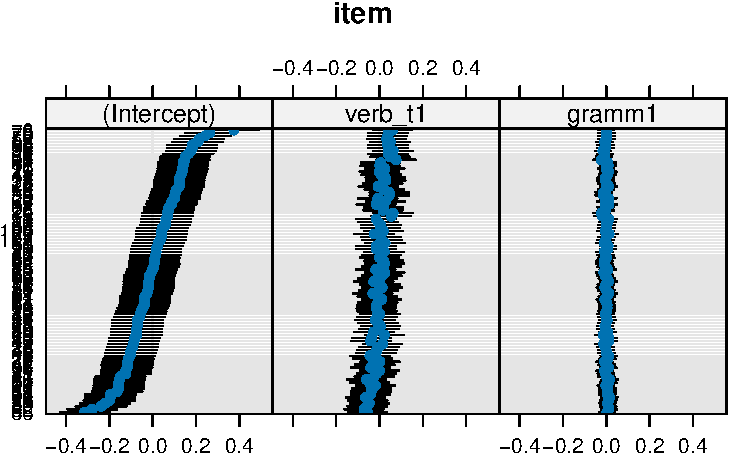
\includegraphics{12-model_selection_example_files/figure-pdf/unnamed-chunk-26-1.pdf}

}

\end{figure}

\hypertarget{by-participant-random-effects-with-1-correlations}{%
\paragraph{by-participant random effects (with +1
correlations)}\label{by-participant-random-effects-with-1-correlations}}

\begin{Shaded}
\begin{Highlighting}[]
\NormalTok{lattice}\SpecialCharTok{::}\FunctionTok{dotplot}\NormalTok{(}\FunctionTok{ranef}\NormalTok{(fit\_verb\_fp\_m1))}\SpecialCharTok{$}\NormalTok{sj}
\end{Highlighting}
\end{Shaded}

\begin{figure}[H]

{\centering 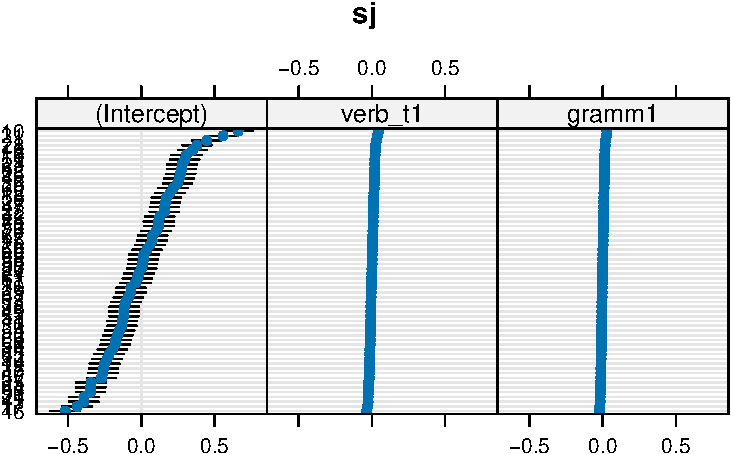
\includegraphics{12-model_selection_example_files/figure-pdf/unnamed-chunk-27-1.pdf}

}

\end{figure}

\hypertarget{alternate-model-2}{%
\subsubsection{Alternate model 2}\label{alternate-model-2}}

\begin{Shaded}
\begin{Highlighting}[]
\NormalTok{fit\_verb\_fp\_m2 }\OtherTok{\textless{}{-}} \FunctionTok{lmer}\NormalTok{(}\FunctionTok{log}\NormalTok{(fp) }\SpecialCharTok{\textasciitilde{}}\NormalTok{ verb\_t}\SpecialCharTok{*}\NormalTok{gramm }\SpecialCharTok{+} 
\NormalTok{                      (}\DecValTok{1} \SpecialCharTok{|}\NormalTok{sj) }\SpecialCharTok{+}
\NormalTok{                      (}\DecValTok{1} \SpecialCharTok{+}\NormalTok{ verb\_t}\SpecialCharTok{+}\NormalTok{gramm}\SpecialCharTok{|}\NormalTok{item),}
                    \AttributeTok{data =}\NormalTok{ df\_biondo,}
                    \AttributeTok{subset =}\NormalTok{ roi }\SpecialCharTok{==} \DecValTok{4}\NormalTok{,}
                    \AttributeTok{control =} \FunctionTok{lmerControl}\NormalTok{(}\AttributeTok{optimizer =} \StringTok{"bobyqa"}\NormalTok{,}
                                          \AttributeTok{optCtrl =} \FunctionTok{list}\NormalTok{(}\AttributeTok{maxfun =} \FloatTok{2e5}\NormalTok{))}
\NormalTok{)}
\end{Highlighting}
\end{Shaded}

\begin{verbatim}
boundary (singular) fit: see help('isSingular')
\end{verbatim}

\hypertarget{repca-1}{%
\paragraph{\texorpdfstring{\texttt{rePCA()}}{rePCA()}}\label{repca-1}}

\begin{Shaded}
\begin{Highlighting}[]
\FunctionTok{summary}\NormalTok{(}\FunctionTok{rePCA}\NormalTok{(fit\_verb\_fp\_m2))}
\end{Highlighting}
\end{Shaded}

\begin{verbatim}
$item
Importance of components:
                         [,1]   [,2] [,3]
Standard deviation     0.3559 0.1297    0
Proportion of Variance 0.8827 0.1173    0
Cumulative Proportion  0.8827 1.0000    1

$sj
Importance of components:
                         [,1]
Standard deviation     0.6441
Proportion of Variance 1.0000
Cumulative Proportion  1.0000
\end{verbatim}

\hypertarget{varcorr-1}{%
\paragraph{\texorpdfstring{\texttt{VarCorr()}}{VarCorr()}}\label{varcorr-1}}

\begin{Shaded}
\begin{Highlighting}[]
\FunctionTok{VarCorr}\NormalTok{(fit\_verb\_fp\_m2)}
\end{Highlighting}
\end{Shaded}

\begin{verbatim}
 Groups   Name        Std.Dev. Corr         
 item     (Intercept) 0.139364              
          verb_t1     0.055805  0.485       
          gramm1      0.020546 -0.097 -0.917
 sj       (Intercept) 0.257648              
 Residual             0.399995              
\end{verbatim}

\begin{itemize}
\tightlist
\item
  by-item slopes for \texttt{gramm} and \texttt{verb\_t} are highly
  correlated
\item
  \texttt{gramm} has least variance, so let's remove it
\end{itemize}

\hypertarget{by-item-random-effects-1}{%
\paragraph{by-item random effects}\label{by-item-random-effects-1}}

\begin{Shaded}
\begin{Highlighting}[]
\NormalTok{lattice}\SpecialCharTok{::}\FunctionTok{dotplot}\NormalTok{(}\FunctionTok{ranef}\NormalTok{(fit\_verb\_fp\_m2))}\SpecialCharTok{$}\NormalTok{item}
\end{Highlighting}
\end{Shaded}

\begin{figure}[H]

{\centering 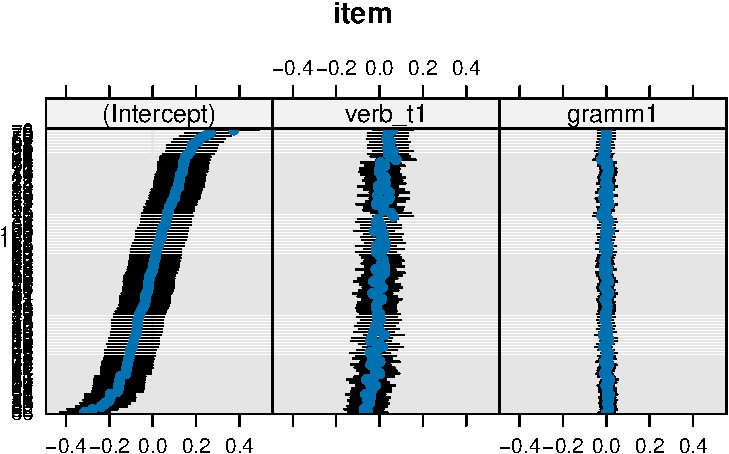
\includegraphics{12-model_selection_example_files/figure-pdf/unnamed-chunk-31-1.pdf}

}

\end{figure}

\hypertarget{alternate-model-3}{%
\subsubsection{Alternate model 3}\label{alternate-model-3}}

\begin{Shaded}
\begin{Highlighting}[]
\NormalTok{fit\_verb\_fp\_m3 }\OtherTok{\textless{}{-}} \FunctionTok{lmer}\NormalTok{(}\FunctionTok{log}\NormalTok{(fp) }\SpecialCharTok{\textasciitilde{}}\NormalTok{ verb\_t}\SpecialCharTok{*}\NormalTok{gramm }\SpecialCharTok{+} 
\NormalTok{                      (}\DecValTok{1} \SpecialCharTok{|}\NormalTok{sj) }\SpecialCharTok{+}
\NormalTok{                      (}\DecValTok{1} \SpecialCharTok{+}\NormalTok{ verb\_t}\SpecialCharTok{|}\NormalTok{item),}
                    \AttributeTok{data =}\NormalTok{ df\_biondo,}
                    \AttributeTok{subset =}\NormalTok{ roi }\SpecialCharTok{==} \DecValTok{4}\NormalTok{,}
                    \AttributeTok{control =} \FunctionTok{lmerControl}\NormalTok{(}\AttributeTok{optimizer =} \StringTok{"bobyqa"}\NormalTok{,}
                                          \AttributeTok{optCtrl =} \FunctionTok{list}\NormalTok{(}\AttributeTok{maxfun =} \FloatTok{2e5}\NormalTok{))}
\NormalTok{)}
\end{Highlighting}
\end{Shaded}

\begin{itemize}
\tightlist
\item
  converged!
\end{itemize}

\hypertarget{repca-2}{%
\paragraph{\texorpdfstring{\texttt{rePCA()}}{rePCA()}}\label{repca-2}}

\begin{Shaded}
\begin{Highlighting}[]
\FunctionTok{summary}\NormalTok{(}\FunctionTok{rePCA}\NormalTok{(fit\_verb\_fp\_m3))}
\end{Highlighting}
\end{Shaded}

\begin{verbatim}
$item
Importance of components:
                         [,1]    [,2]
Standard deviation     0.3553 0.10311
Proportion of Variance 0.9223 0.07768
Cumulative Proportion  0.9223 1.00000

$sj
Importance of components:
                         [,1]
Standard deviation     0.6438
Proportion of Variance 1.0000
Cumulative Proportion  1.0000
\end{verbatim}

\hypertarget{varcorr-2}{%
\paragraph{\texorpdfstring{\texttt{VarCorr()}}{VarCorr()}}\label{varcorr-2}}

\begin{Shaded}
\begin{Highlighting}[]
\FunctionTok{VarCorr}\NormalTok{(fit\_verb\_fp\_m3)}
\end{Highlighting}
\end{Shaded}

\begin{verbatim}
 Groups   Name        Std.Dev. Corr 
 item     (Intercept) 0.139365      
          verb_t1     0.050134 0.542
 sj       (Intercept) 0.257714      
 Residual             0.400315      
\end{verbatim}

\hypertarget{alternate-model-4}{%
\subsubsection{Alternate model 4}\label{alternate-model-4}}

\begin{itemize}
\tightlist
\item
  but we might've also decided to remove \texttt{verb\_t}, so let's run
  that model
\end{itemize}

\begin{Shaded}
\begin{Highlighting}[]
\NormalTok{fit\_verb\_fp\_m4 }\OtherTok{\textless{}{-}} \FunctionTok{lmer}\NormalTok{(}\FunctionTok{log}\NormalTok{(fp) }\SpecialCharTok{\textasciitilde{}}\NormalTok{ verb\_t}\SpecialCharTok{*}\NormalTok{gramm }\SpecialCharTok{+} 
\NormalTok{                      (}\DecValTok{1} \SpecialCharTok{|}\NormalTok{sj) }\SpecialCharTok{+}
\NormalTok{                      (}\DecValTok{1} \SpecialCharTok{+}\NormalTok{ gramm}\SpecialCharTok{|}\NormalTok{item),}
                    \AttributeTok{data =}\NormalTok{ df\_biondo,}
                    \AttributeTok{subset =}\NormalTok{ roi }\SpecialCharTok{==} \DecValTok{4}\NormalTok{,}
                    \AttributeTok{control =} \FunctionTok{lmerControl}\NormalTok{(}\AttributeTok{optimizer =} \StringTok{"bobyqa"}\NormalTok{,}
                                          \AttributeTok{optCtrl =} \FunctionTok{list}\NormalTok{(}\AttributeTok{maxfun =} \FloatTok{2e5}\NormalTok{))}
\NormalTok{)}
\end{Highlighting}
\end{Shaded}

\begin{verbatim}
boundary (singular) fit: see help('isSingular')
\end{verbatim}

\begin{itemize}
\tightlist
\item
  does not converge, so we're justified in keeping by-item
  \texttt{verb\_t} slopes
\end{itemize}

\hypertarget{final-model}{%
\subsection{Final model}\label{final-model}}

\begin{itemize}
\tightlist
\item
  the final model name should be some sort of convention to make your
  life easier

  \begin{itemize}
  \tightlist
  \item
    so remove model index
  \end{itemize}
\end{itemize}

\begin{Shaded}
\begin{Highlighting}[]
\NormalTok{fit\_verb\_fp }\OtherTok{\textless{}{-}}\NormalTok{ fit\_verb\_fp\_m3}
\end{Highlighting}
\end{Shaded}

\hypertarget{by-item-random-effects-2}{%
\paragraph{by-item random effects}\label{by-item-random-effects-2}}

\begin{Shaded}
\begin{Highlighting}[]
\NormalTok{lattice}\SpecialCharTok{::}\FunctionTok{dotplot}\NormalTok{(}\FunctionTok{ranef}\NormalTok{(fit\_verb\_fp))}\SpecialCharTok{$}\NormalTok{sj}
\end{Highlighting}
\end{Shaded}

\begin{figure}[H]

{\centering 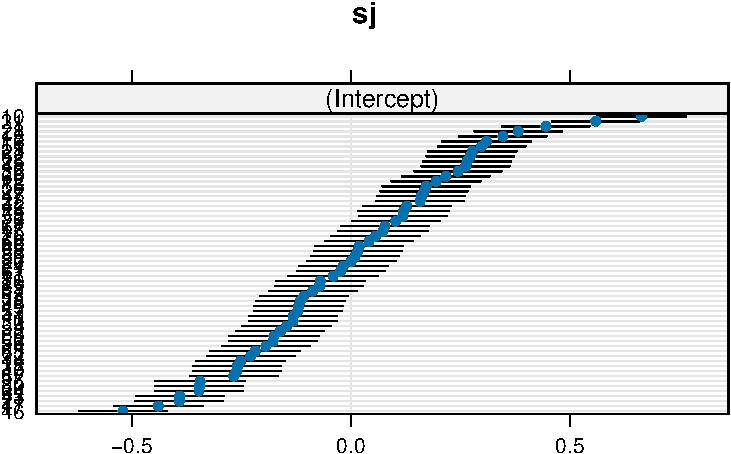
\includegraphics{12-model_selection_example_files/figure-pdf/unnamed-chunk-37-1.pdf}

}

\end{figure}

\hypertarget{by-participant-random-effects}{%
\paragraph{by-participant random
effects}\label{by-participant-random-effects}}

\begin{Shaded}
\begin{Highlighting}[]
\NormalTok{lattice}\SpecialCharTok{::}\FunctionTok{dotplot}\NormalTok{(}\FunctionTok{ranef}\NormalTok{(fit\_verb\_fp))}\SpecialCharTok{$}\NormalTok{item}
\end{Highlighting}
\end{Shaded}

\begin{figure}[H]

{\centering 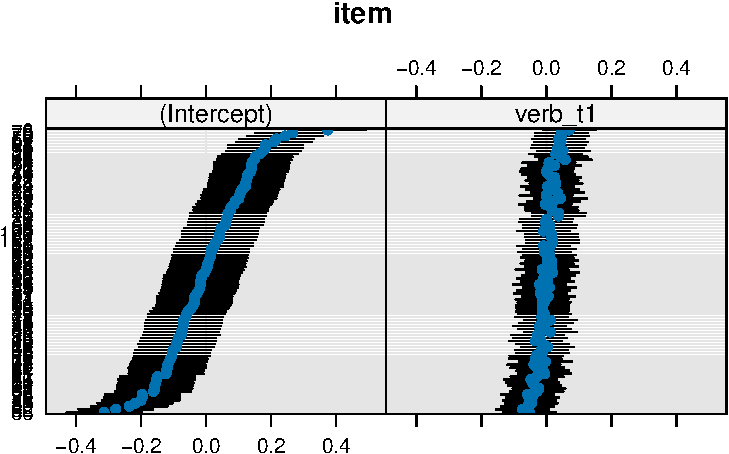
\includegraphics{12-model_selection_example_files/figure-pdf/unnamed-chunk-38-1.pdf}

}

\end{figure}

\hypertarget{summary}{%
\paragraph{\texorpdfstring{\texttt{summary()}}{summary()}}\label{summary}}

\begin{Shaded}
\begin{Highlighting}[]
\FunctionTok{summary}\NormalTok{(fit\_verb\_fp)}
\end{Highlighting}
\end{Shaded}

\begin{verbatim}
Linear mixed model fit by REML. t-tests use Satterthwaite's method [
lmerModLmerTest]
Formula: log(fp) ~ verb_t * gramm + (1 | sj) + (1 + verb_t | item)
   Data: df_biondo
Control: lmerControl(optimizer = "bobyqa", optCtrl = list(maxfun = 200000))
 Subset: roi == 4

REML criterion at convergence: 4216.2

Scaled residuals: 
    Min      1Q  Median      3Q     Max 
-4.1758 -0.6096 -0.0227  0.6060  4.0568 

Random effects:
 Groups   Name        Variance Std.Dev. Corr
 item     (Intercept) 0.019423 0.13936      
          verb_t1     0.002513 0.05013  0.54
 sj       (Intercept) 0.066417 0.25771      
 Residual             0.160252 0.40032      
Number of obs: 3795, groups:  item, 96; sj, 60

Fixed effects:
                  Estimate  Std. Error          df t value             Pr(>|t|)
(Intercept)       5.956384    0.036763   79.243183 162.021 < 0.0000000000000002
verb_t1           0.061733    0.013971   93.410602   4.419            0.0000267
gramm1            0.003298    0.012999 3544.451823   0.254                 0.80
verb_t1:gramm1   -0.014380    0.025998 3544.762347  -0.553                 0.58
                  
(Intercept)    ***
verb_t1        ***
gramm1            
verb_t1:gramm1    
---
Signif. codes:  0 '***' 0.001 '**' 0.01 '*' 0.05 '.' 0.1 ' ' 1

Correlation of Fixed Effects:
            (Intr) vrb_t1 gramm1
verb_t1      0.077              
gramm1       0.000 -0.002       
vrb_t1:grm1  0.000  0.002  0.000
\end{verbatim}

\begin{itemize}
\tightlist
\item
  IMPORTANTLY, only look at the fixed effects after you've got your
  final model!!!!

  \begin{itemize}
  \tightlist
  \item
    i.e., run model -\textgreater{} convergence error -\textgreater{}
    \texttt{rePCA()} + \texttt{VarCorr()} -\textgreater{} run model
    -\textgreater{} \ldots{} -\textgreater{} converges -\textgreater{}
    only NOW run \texttt{summary(model)}
  \end{itemize}
\end{itemize}

\hypertarget{comparing-to-bad-models}{%
\section{Comparing to `bad' models}\label{comparing-to-bad-models}}

\begin{itemize}
\tightlist
\item
  let's compare our final model to our `bad' models

  \begin{itemize}
  \tightlist
  \item
    random intercepts-only model (overconfident)
  \item
    maximal model (underconfident)
  \end{itemize}
\end{itemize}

\hypertarget{random-intercepts-only}{%
\subsection{Random-intercepts only}\label{random-intercepts-only}}

\begin{Shaded}
\begin{Highlighting}[]
\NormalTok{fit\_verb\_fp\_intercepts }\OtherTok{\textless{}{-}} \FunctionTok{lmer}\NormalTok{(}\FunctionTok{log}\NormalTok{(fp) }\SpecialCharTok{\textasciitilde{}}\NormalTok{ verb\_t}\SpecialCharTok{*}\NormalTok{gramm }\SpecialCharTok{+} 
\NormalTok{                      (}\DecValTok{1} \SpecialCharTok{|}\NormalTok{sj) }\SpecialCharTok{+}
\NormalTok{                      (}\DecValTok{1} \SpecialCharTok{|}\NormalTok{item),}
                    \AttributeTok{data =}\NormalTok{ df\_biondo,}
                    \AttributeTok{subset =}\NormalTok{ roi }\SpecialCharTok{==} \DecValTok{4}
\NormalTok{)}
\end{Highlighting}
\end{Shaded}

\begin{itemize}
\tightlist
\item
  converges
\end{itemize}

\begin{Shaded}
\begin{Highlighting}[]
\NormalTok{sum\_fit\_verb\_fp }\OtherTok{\textless{}{-}}
  \FunctionTok{tidy}\NormalTok{(fit\_verb\_fp,}
     \AttributeTok{effects =} \StringTok{"fixed"}\NormalTok{) }\SpecialCharTok{|\textgreater{}} 
  \FunctionTok{as\_tibble}\NormalTok{() }\SpecialCharTok{|\textgreater{}} 
  \FunctionTok{mutate}\NormalTok{(}\AttributeTok{p\_value =} \FunctionTok{format\_pval}\NormalTok{(p.value),}
         \AttributeTok{model =} \StringTok{"parsimonious"}\NormalTok{) }

\NormalTok{sum\_fit\_verb\_fp\_mm }\OtherTok{\textless{}{-}}
  \FunctionTok{tidy}\NormalTok{(fit\_verb\_fp\_mm,}
     \AttributeTok{effects =} \StringTok{"fixed"}\NormalTok{) }\SpecialCharTok{|\textgreater{}} 
  \FunctionTok{as\_tibble}\NormalTok{() }\SpecialCharTok{|\textgreater{}} 
  \FunctionTok{mutate}\NormalTok{(}\AttributeTok{p\_value =} \FunctionTok{format\_pval}\NormalTok{(p.value),}
         \AttributeTok{model =} \StringTok{"maximal"}\NormalTok{) }

\NormalTok{sum\_fit\_verb\_fp\_intercepts }\OtherTok{\textless{}{-}}
  \FunctionTok{tidy}\NormalTok{(fit\_verb\_fp\_intercepts,}
     \AttributeTok{effects =} \StringTok{"fixed"}\NormalTok{) }\SpecialCharTok{|\textgreater{}} 
  \FunctionTok{as\_tibble}\NormalTok{() }\SpecialCharTok{|\textgreater{}} 
  \FunctionTok{mutate}\NormalTok{(}\AttributeTok{p\_value =} \FunctionTok{format\_pval}\NormalTok{(p.value),}
         \AttributeTok{model =} \StringTok{"intercepts"}\NormalTok{)}
\end{Highlighting}
\end{Shaded}

\hypertarget{coefficient-estimates}{%
\subsection{coefficient estimates}\label{coefficient-estimates}}

\begin{Shaded}
\begin{Highlighting}[]
\FunctionTok{rbind}\NormalTok{(sum\_fit\_verb\_fp, sum\_fit\_verb\_fp\_intercepts, sum\_fit\_verb\_fp\_mm) }\SpecialCharTok{|\textgreater{}} 
  \FunctionTok{select}\NormalTok{(term, estimate, model) }\SpecialCharTok{|\textgreater{}}
  \FunctionTok{mutate}\NormalTok{(}\AttributeTok{estimate =} \FunctionTok{round}\NormalTok{(estimate,}\DecValTok{4}\NormalTok{)) }\SpecialCharTok{|\textgreater{}} 
  \FunctionTok{pivot\_wider}\NormalTok{(}
    \AttributeTok{id\_cols =} \FunctionTok{c}\NormalTok{(term),}
    \AttributeTok{names\_from =}\NormalTok{ model,}
    \AttributeTok{values\_from =}\NormalTok{ estimate}
\NormalTok{  ) }\SpecialCharTok{|\textgreater{}} 
  \FunctionTok{mutate}\NormalTok{(}\AttributeTok{measure =} \StringTok{"estimate"}\NormalTok{) }\SpecialCharTok{|\textgreater{}} 
  \FunctionTok{kable}\NormalTok{() }\SpecialCharTok{|\textgreater{}} 
  \FunctionTok{kable\_styling}\NormalTok{()}
\end{Highlighting}
\end{Shaded}

\hypertarget{tbl-estimates}{}
\begin{longtable}[t]{lrrrl}
\caption{\label{tbl-estimates}Coefficient estimates for our parsimonious model, a random-intercepts
only model, and a maximal model }\tabularnewline

\toprule
term & parsimonious & intercepts & maximal & measure\\
\midrule
(Intercept) & 5.9564 & 5.9564 & 5.9564 & estimate\\
verb\_t1 & 0.0617 & 0.0619 & 0.0617 & estimate\\
gramm1 & 0.0033 & 0.0032 & 0.0034 & estimate\\
verb\_t1:gramm1 & -0.0144 & -0.0143 & -0.0142 & estimate\\
\bottomrule
\end{longtable}

\hypertarget{standard-error}{%
\subsection{standard error}\label{standard-error}}

\begin{Shaded}
\begin{Highlighting}[]
\FunctionTok{rbind}\NormalTok{(sum\_fit\_verb\_fp, sum\_fit\_verb\_fp\_intercepts, sum\_fit\_verb\_fp\_mm) }\SpecialCharTok{|\textgreater{}} 
  \FunctionTok{select}\NormalTok{(term, std.error, model) }\SpecialCharTok{|\textgreater{}}
  \FunctionTok{mutate}\NormalTok{(}\AttributeTok{std.error =} \FunctionTok{round}\NormalTok{(std.error,}\DecValTok{4}\NormalTok{)) }\SpecialCharTok{|\textgreater{}} 
  \FunctionTok{pivot\_wider}\NormalTok{(}
    \AttributeTok{id\_cols =} \FunctionTok{c}\NormalTok{(term),}
    \AttributeTok{names\_from =}\NormalTok{ model,}
    \AttributeTok{values\_from =}\NormalTok{ std.error}
\NormalTok{  ) }\SpecialCharTok{|\textgreater{}} 
  \FunctionTok{mutate}\NormalTok{(}\AttributeTok{measure =} \StringTok{"std.error"}\NormalTok{) }\SpecialCharTok{|\textgreater{}} 
  \FunctionTok{kable}\NormalTok{() }\SpecialCharTok{|\textgreater{}} 
  \FunctionTok{kable\_styling}\NormalTok{()}
\end{Highlighting}
\end{Shaded}

\hypertarget{tbl-std_error}{}
\begin{longtable}[t]{lrrrl}
\caption{\label{tbl-std_error}Standard error of coefficient estimates for our parsimonious model, a
random-intercepts only model, and a maximal model }\tabularnewline

\toprule
term & parsimonious & intercepts & maximal & measure\\
\midrule
(Intercept) & 0.0368 & 0.0368 & 0.0367 & std.error\\
verb\_t1 & 0.0140 & 0.0130 & 0.0144 & std.error\\
gramm1 & 0.0130 & 0.0130 & 0.0133 & std.error\\
verb\_t1:gramm1 & 0.0260 & 0.0260 & 0.0278 & std.error\\
\bottomrule
\end{longtable}

\begin{itemize}
\tightlist
\item
  standard error (\textbackslash{}\(SE = \frac{\sigma}{\sqrt{n}}\\\)) is
  a measure of uncertainty

  \begin{itemize}
  \tightlist
  \item
    larger values reflect greater uncertainty
  \item
    because \(n\) is in the denominator, SE gets smaller with more
    observations
  \end{itemize}
\item
  compared to our parsimonious model with by-item varying
  \texttt{verb\_t} slopes:

  \begin{itemize}
  \tightlist
  \item
    smaller SE for our overconfident (intercepts) model
  \item
    larger SE for our underconfident (maximal) model
  \item
    but only for the estimate also included in the random effects
  \end{itemize}
\end{itemize}

\hypertarget{t-values}{%
\subsection{t-values}\label{t-values}}

\begin{Shaded}
\begin{Highlighting}[]
\FunctionTok{rbind}\NormalTok{(sum\_fit\_verb\_fp, sum\_fit\_verb\_fp\_intercepts, sum\_fit\_verb\_fp\_mm) }\SpecialCharTok{|\textgreater{}} 
  \FunctionTok{select}\NormalTok{(term, statistic, model) }\SpecialCharTok{|\textgreater{}}
  \FunctionTok{mutate}\NormalTok{(}\AttributeTok{statistic =} \FunctionTok{round}\NormalTok{(statistic,}\DecValTok{4}\NormalTok{)) }\SpecialCharTok{|\textgreater{}} 
  \FunctionTok{pivot\_wider}\NormalTok{(}
    \AttributeTok{id\_cols =} \FunctionTok{c}\NormalTok{(term),}
    \AttributeTok{names\_from =}\NormalTok{ model,}
    \AttributeTok{values\_from =}\NormalTok{ statistic}
\NormalTok{  ) }\SpecialCharTok{|\textgreater{}} 
  \FunctionTok{mutate}\NormalTok{(}\AttributeTok{measure =} \StringTok{"statistic"}\NormalTok{) }\SpecialCharTok{|\textgreater{}} 
  \FunctionTok{kable}\NormalTok{() }\SpecialCharTok{|\textgreater{}} 
  \FunctionTok{kable\_styling}\NormalTok{()}
\end{Highlighting}
\end{Shaded}

\hypertarget{tbl-t_value}{}
\begin{longtable}[t]{lrrrl}
\caption{\label{tbl-t_value}t-values of each estimates for our parsimonious model, a
random-intercepts only model, and a maximal model }\tabularnewline

\toprule
term & parsimonious & intercepts & maximal & measure\\
\midrule
(Intercept) & 162.0213 & 161.9025 & 162.1605 & statistic\\
verb\_t1 & 4.4188 & 4.7517 & 4.2982 & statistic\\
gramm1 & 0.2537 & 0.2466 & 0.2542 & statistic\\
verb\_t1:gramm1 & -0.5531 & -0.5496 & -0.5108 & statistic\\
\bottomrule
\end{longtable}

\begin{itemize}
\tightlist
\item
  t-value (\textbackslash{}\(t = \frac{\bar{x}_1 - \bar{x}_2}{SE}\\\))
  is a measure of uncertainty

  \begin{itemize}
  \tightlist
  \item
    larger values reflect greater effect
  \item
    more \(n\) increases \(t\)
  \end{itemize}
\item
  again, \texttt{verb\_t}: \(t_{max}\) \textless{} \(t_{pars}\)
  \textless{} \(t_{int}\)
\end{itemize}

\hypertarget{degrees-of-freedom}{%
\subsection{degrees of freedom}\label{degrees-of-freedom}}

\begin{Shaded}
\begin{Highlighting}[]
\FunctionTok{rbind}\NormalTok{(sum\_fit\_verb\_fp, sum\_fit\_verb\_fp\_intercepts, sum\_fit\_verb\_fp\_mm) }\SpecialCharTok{|\textgreater{}} 
  \FunctionTok{select}\NormalTok{(term, df, model) }\SpecialCharTok{|\textgreater{}}
  \FunctionTok{mutate}\NormalTok{(}\AttributeTok{df =} \FunctionTok{round}\NormalTok{(df,}\DecValTok{4}\NormalTok{)) }\SpecialCharTok{|\textgreater{}} 
  \FunctionTok{pivot\_wider}\NormalTok{(}
    \AttributeTok{id\_cols =} \FunctionTok{c}\NormalTok{(term),}
    \AttributeTok{names\_from =}\NormalTok{ model,}
    \AttributeTok{values\_from =}\NormalTok{ df}
\NormalTok{  ) }\SpecialCharTok{|\textgreater{}} 
  \FunctionTok{mutate}\NormalTok{(}\AttributeTok{measure =} \StringTok{"df"}\NormalTok{) }\SpecialCharTok{|\textgreater{}} 
  \FunctionTok{kable}\NormalTok{() }\SpecialCharTok{|\textgreater{}} 
  \FunctionTok{kable\_styling}\NormalTok{()}
\end{Highlighting}
\end{Shaded}

\hypertarget{tbl-df}{}
\begin{longtable}[t]{lrrrl}
\caption{\label{tbl-df}Degrees of freedom of each estimates for our parsimonious model, a
random-intercepts only model, and a maximal model }\tabularnewline

\toprule
term & parsimonious & intercepts & maximal & measure\\
\midrule
(Intercept) & 79.2432 & 79.2008 & 79.1789 & df\\
verb\_t1 & 93.4106 & 3637.1332 & 71.4326 & df\\
gramm1 & 3544.4518 & 3637.1834 & 180.0819 & df\\
verb\_t1:gramm1 & 3544.7623 & 3637.1023 & 91.8570 & df\\
\bottomrule
\end{longtable}

\begin{itemize}
\tightlist
\item
  degrees of freedom: not trivially defined in mixed models; we're using
  Satterthwaite approximiation (default in \texttt{lmerTest::lmer()})

  \begin{itemize}
  \tightlist
  \item
    larger degrees of freedom corresponds to larger \(n\)
  \item
    including more random effects reduces our \(n\) and therefore
    reduces \(df\)
  \end{itemize}
\item
  again, \texttt{verb\_t}: \(df_{max}\) \textless{} \(df_{pars}\)
  \textless{} \(df_{int}\)

  \begin{itemize}
  \tightlist
  \item
    and large differences between our maximal model and the other two
    for other terms
  \end{itemize}
\end{itemize}

\hypertarget{p-values}{%
\subsection{p-values}\label{p-values}}

\begin{Shaded}
\begin{Highlighting}[]
\FunctionTok{rbind}\NormalTok{(sum\_fit\_verb\_fp, sum\_fit\_verb\_fp\_intercepts, sum\_fit\_verb\_fp\_mm) }\SpecialCharTok{|\textgreater{}} 
  \FunctionTok{select}\NormalTok{(term, p.value, model) }\SpecialCharTok{|\textgreater{}}
  \FunctionTok{mutate}\NormalTok{(}\AttributeTok{p.value =} \FunctionTok{round}\NormalTok{(p.value, }\DecValTok{8}\NormalTok{)) }\SpecialCharTok{|\textgreater{}} 
  \FunctionTok{pivot\_wider}\NormalTok{(}
    \AttributeTok{id\_cols =} \FunctionTok{c}\NormalTok{(term),}
    \AttributeTok{names\_from =}\NormalTok{ model,}
    \AttributeTok{values\_from =}\NormalTok{ p.value}
\NormalTok{  ) }\SpecialCharTok{|\textgreater{}} 
  \FunctionTok{mutate}\NormalTok{(}\AttributeTok{measure =} \StringTok{"p.value"}\NormalTok{) }\SpecialCharTok{|\textgreater{}} 
  \FunctionTok{kable}\NormalTok{() }\SpecialCharTok{|\textgreater{}} 
  \FunctionTok{kable\_styling}\NormalTok{()}
\end{Highlighting}
\end{Shaded}

\hypertarget{tbl-p_value}{}
\begin{longtable}[t]{lrrrl}
\caption{\label{tbl-p_value}p-values of coefficient estimates for our parsimonious model, a
random-intercepts only model, and a maximal model }\tabularnewline

\toprule
term & parsimonious & intercepts & maximal & measure\\
\midrule
(Intercept) & 0.0000000 & 0.0000000 & 0.0000000 & p.value\\
verb\_t1 & 0.0000267 & 0.0000021 & 0.0000535 & p.value\\
gramm1 & 0.7997645 & 0.8052568 & 0.7996177 & p.value\\
verb\_t1:gramm1 & 0.5802114 & 0.5826522 & 0.6107494 & p.value\\
\bottomrule
\end{longtable}

\begin{itemize}
\tightlist
\item
  p-values: inversely related to t-values (larger t-values = smaller
  p-values)
\item
  again, \texttt{verb\_t}: \(p_{max}\) \textless{} \(p_{pars}\)
  \textless{} \(p_{int}\)

  \begin{itemize}
  \tightlist
  \item
    this would be important for `signicance' if the values were closer
    to the convential alpha-levels (p \textless{} .05, p \textless{}
    .01, p \textless{} .001)
  \item
    but here the different random effects structures don't qualitatively
    change (all are \textless{} .001)
  \end{itemize}
\item
  this is not always the case, however!

  \begin{itemize}
  \tightlist
  \item
    this is why we do not peek at the fixed effects until we have our
    final model
  \item
    we don't want to be influenced (consciously or not) by seeing small
    p-values in one model but not another
  \end{itemize}
\end{itemize}

\hypertarget{reporting}{%
\section{Reporting}\label{reporting}}

\begin{itemize}
\tightlist
\item
  in Data Analysis section, e.g.,
\end{itemize}

\begin{quote}
We included Time Reference (past, future), and Verb Match (match,
mismatch) as fixed-effect factors in the models used to investigate the
processing of past--future violations (Q1), by adopting sum contrast
coding (Schad et al., 2020): past and match conditions were coded as
--.5. while future and mismatch conditions were coded as .5.
{[}\ldots{]} Moreover, we included crossed random intercepts and random
slopes for all fixed-effect parameters for subject and item grouping
factors (Barr et al., 2013) in all models.

We reduced the complexity of the random effect structure of the maximal
model by performing a principal component analysis so as to identify the
most parsimonious model properly supported by the data (Bates et al.,
2015). {[}\ldots{]} all reading time data were log transformed before
performing the analyses.

--- Biondo et al. (2022), p.~9
\end{quote}

\hypertarget{formatted-p-values}{%
\subsection{Formatted p-values}\label{formatted-p-values}}

\begin{itemize}
\tightlist
\item
  we can use the \texttt{format\_pval()} function defined earlier to
  produce formatted p-values
\end{itemize}

\begin{Shaded}
\begin{Highlighting}[]
  \FunctionTok{tidy}\NormalTok{(fit\_verb\_fp,}
     \AttributeTok{effects =} \StringTok{"fixed"}\NormalTok{) }\SpecialCharTok{|\textgreater{}} 
  \FunctionTok{as\_tibble}\NormalTok{() }\SpecialCharTok{|\textgreater{}} 
  \FunctionTok{mutate}\NormalTok{(}\AttributeTok{p\_value =} \FunctionTok{format\_pval}\NormalTok{(p.value)) }\SpecialCharTok{|\textgreater{}} 
  \FunctionTok{select}\NormalTok{(}\SpecialCharTok{{-}}\NormalTok{p.value) }\SpecialCharTok{|\textgreater{}} 
  \FunctionTok{kable}\NormalTok{() }\SpecialCharTok{|\textgreater{}} 
  \FunctionTok{kable\_styling}\NormalTok{()}
\end{Highlighting}
\end{Shaded}

\hypertarget{tbl-format_pval}{}
\begin{longtable}[t]{llrrrrl}
\caption{\label{tbl-format_pval}Table with formatted p-values from \texttt{format\_pval()} }\tabularnewline

\toprule
effect & term & estimate & std.error & statistic & df & p\_value\\
\midrule
fixed & (Intercept) & 5.9563839 & 0.0367630 & 162.0213386 & 79.24318 & < .001\\
fixed & verb\_t1 & 0.0617330 & 0.0139706 & 4.4187860 & 93.41060 & < .001\\
fixed & gramm1 & 0.0032976 & 0.0129994 & 0.2536709 & 3544.45182 & 0.800\\
fixed & verb\_t1:gramm1 & -0.0143804 & 0.0259984 & -0.5531269 & 3544.76235 & 0.580\\
\bottomrule
\end{longtable}

\hypertarget{learning-objectives-1}{%
\section*{Learning objectives 🏁}\label{learning-objectives-1}}

Today we\ldots{}

\begin{itemize}
\tightlist
\item
  applied remedies for nonconvergence ✅
\item
  reduced our RES with a data-driven approach ✅
\item
  compared a parsimonious model to maximal and intercept-only models ✅
\end{itemize}

\hypertarget{important-terms}{%
\section*{Important terms}\label{important-terms}}
\addcontentsline{toc}{section}{Important terms}

\begin{longtable*}{lll}
\toprule
Term & Definition & Equation/Code \\ 
\midrule
linear mixed (effects) model & NA & NA \\ 
\bottomrule
\end{longtable*}

\hypertarget{references}{%
\section*{References}\label{references}}

\hypertarget{refs}{}
\begin{CSLReferences}{1}{0}
\leavevmode\vadjust pre{\hypertarget{ref-barr_random_maximal_2013}{}}%
Barr, D. J., Levy, R., Scheepers, C., \& Tily, H. J. (2013). Random
effects structure for confirmatory hypothesis testing: {Keep} it
maximal. \emph{Journal of Memory and Language}, \emph{68}(3), 255--278.
\url{https://doi.org/10.1016/j.jml.2012.11.001}

\leavevmode\vadjust pre{\hypertarget{ref-bates_parsimonious_2015}{}}%
Bates, D., Kliegl, R., Vasishth, S., \& Baayen, H. (2015). Parsimonious
{Mixed Models}. \emph{arXiv Preprint}, 1--27.
\url{https://doi.org/10.48550/arXiv.1506.04967}

\leavevmode\vadjust pre{\hypertarget{ref-biondo_yesterday_2022}{}}%
Biondo, N., Soilemezidi, M., \& Mancini, S. (2022). Yesterday is
history, tomorrow is a mystery: {An} eye-tracking investigation of the
processing of past and future time reference during sentence reading.
\emph{Journal of Experimental Psychology: Learning, Memory, and
Cognition}, \emph{48}(7), 1001--1018.
\url{https://doi.org/10.1037/xlm0001053}

\leavevmode\vadjust pre{\hypertarget{ref-brauer_linear_2018}{}}%
Brauer, M., \& Curtin, J. J. (2018). Linear mixed-effects models and the
analysis of nonindependent data: {A} unified framework to analyze
categorical and continuous independent variables that vary
within-subjects and/or within-items. \emph{Psychological Methods},
\emph{23}(3), 389--411. \url{https://doi.org/10.1037/met0000159}

\leavevmode\vadjust pre{\hypertarget{ref-meteyard_best_2020}{}}%
Meteyard, L., \& Davies, R. A. I. (2020). Best practice guidance for
linear mixed-effects models in psychological science. \emph{Journal of
Memory and Language}, \emph{112}, 104092.
\url{https://doi.org/10.1016/j.jml.2020.104092}

\leavevmode\vadjust pre{\hypertarget{ref-sonderegger_regression_2023}{}}%
Sonderegger, M. (2023). \emph{Regression {Modeling} for {Linguistic
Data}}.

\leavevmode\vadjust pre{\hypertarget{ref-winter_statistics_2019}{}}%
Winter, B. (2019). Statistics for {Linguists}: {An Introduction Using
R}. In \emph{Statistics for Linguists: An Introduction Using R}.
{Routledge}. \url{https://doi.org/10.4324/9781315165547}

\end{CSLReferences}



\end{document}
